\newpage
\section{Elliptic Curves}
\index{Elliptic curves}
\hypertarget{ellcurve}{}
(Filipovics B. / Esslinger B. / Oyono R., April 2000, Update Dec. 2001,
June 2002)

\subsection{Elliptic curce cryptography --- a high-performance substitute for RSA?}

In the financial business secure and efficient data transfer is essential.
In particular, the RSA algorithm is used in many applications. Although the
security of RSA is beyond doubt, the evolution in computing power has
caused a growth in the necessary key length.  Today, 1024-bit RSA-keys are
standard, but the The GISA\index{GISA} (German Information Security Agency)
recommends the usage of 2048-bit keys from 2006 on (compare
section~\ref{SecurityRSA}).  The fact that most chips on smart cards cannot
process keys extending 1024 bit shows that there is a need for
alternatives. Elliptic curve cryptography (ECC) can be an such an
alternative in the field of asymmetric cryptography.

The efficiency of a cryptographic algorithm depends on the key length and
the calculation effort that is necessary to provide a prescribed level of
security. The major advantage of ECC compared to RSA is that it requires
much shorter key lengths. If we assume that the computing power increases
by Moore�s law (i.~e.\ it doubles every 18 months), then the evolution of
the key lengths for secure communication will be as
figure~\ref{ThousandBitMultiplications} (source: Arjen Lenstra und Eric
Verheul:
\href{http://cryptosavvy.com/table.htm}{\texttt{http://cryptosavvy.com/table.htm}}).

% -> Figure 1
\begin{figure}[h]
\begin{center}
\vspace{1.5cm}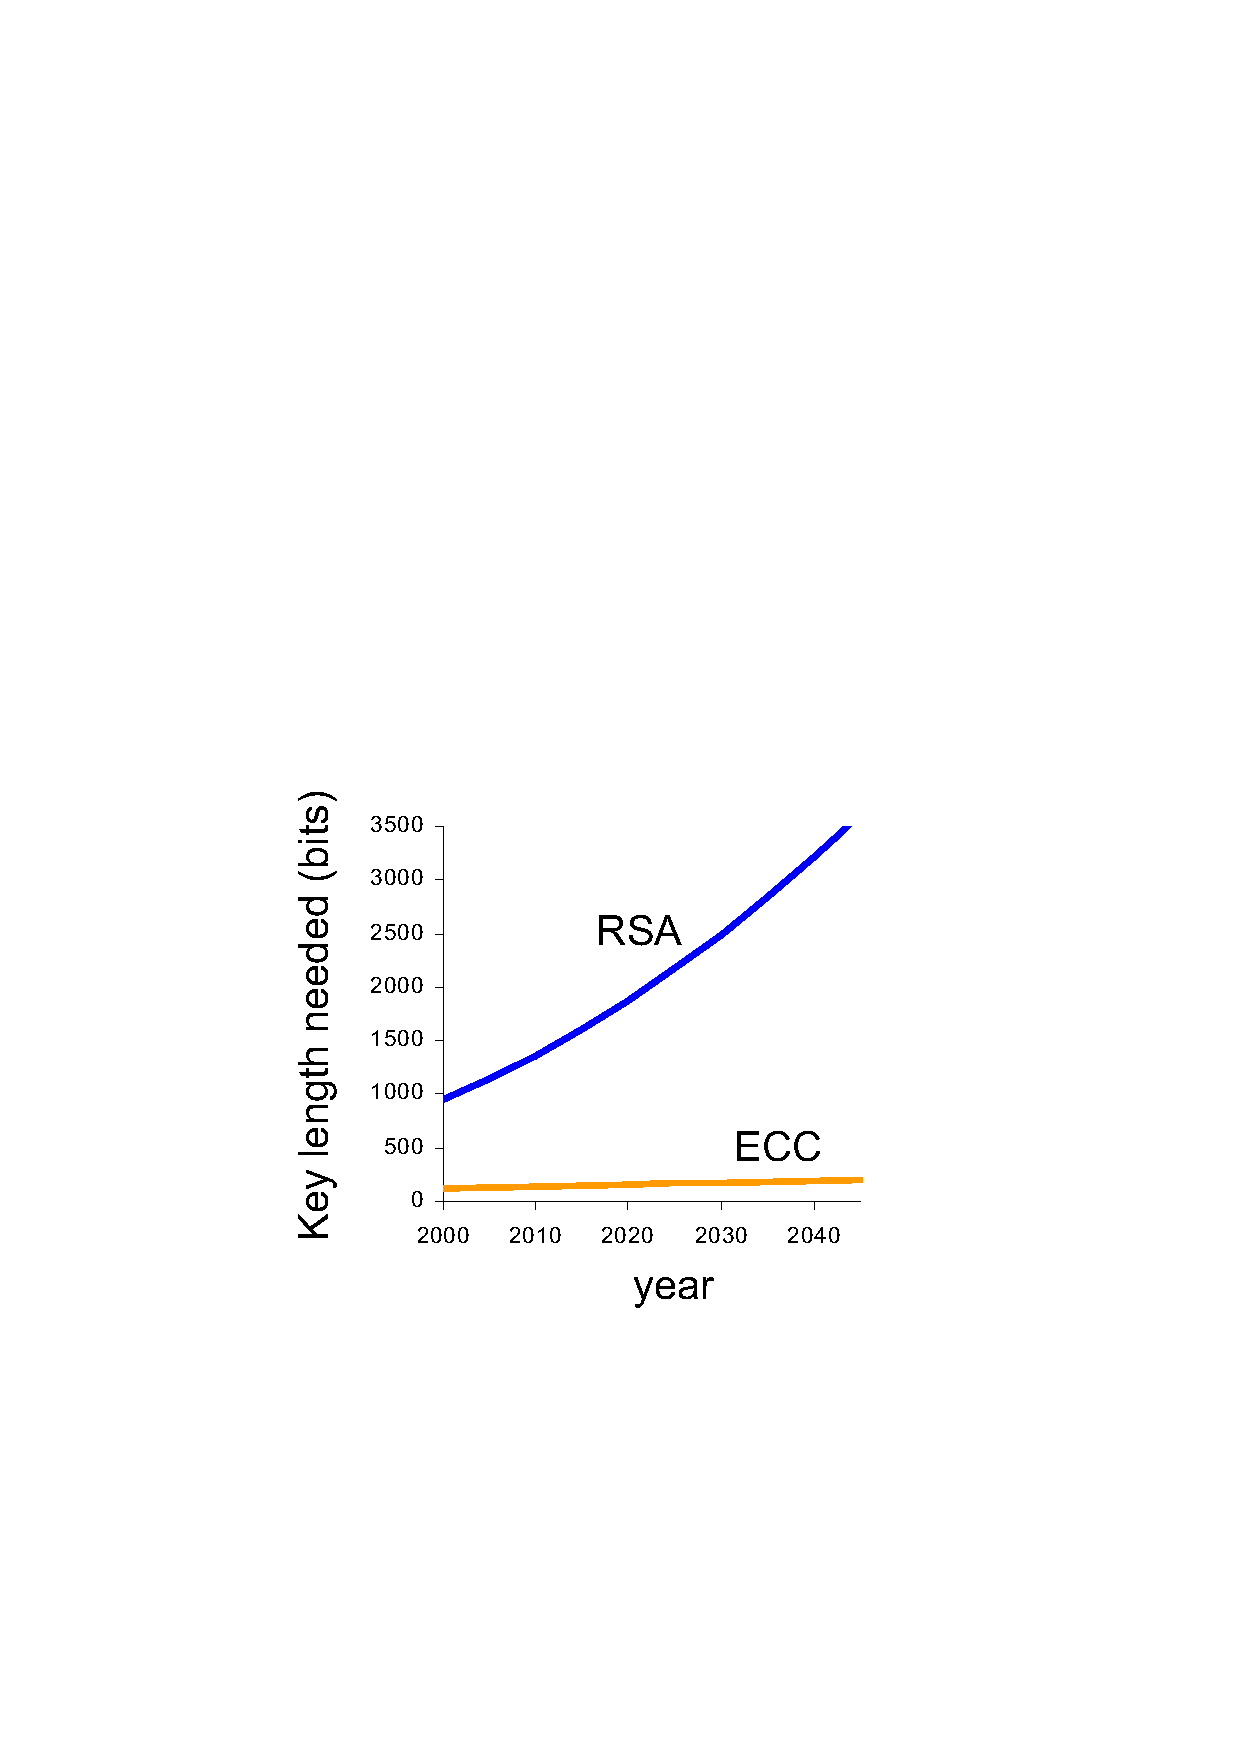
\includegraphics[scale=0.75]{figures/RSAKeylength}
\caption{Comparison of signing and verification time for RSA and Elliptic Curves} 
\label{RSAKeylength}
\end{center}
\end{figure}

In addition, a digital signature can be processed 10-times faster with ECC
than with RSA.  However, verification of a given signature is still more
efficient with RSA than with ECC. Refer to
figure~\ref{ThousandBitMultiplications} (source: Dr.~J.\ Merkle, Elliptic
Curve Cryptography Workshop, 2001) for a comparison.  The reason is that
RSA public keys can be chosen relatively small as long as the secret key is
sufficiently long.

% -> Figure 2
\begin{figure}[h]
\begin{center}
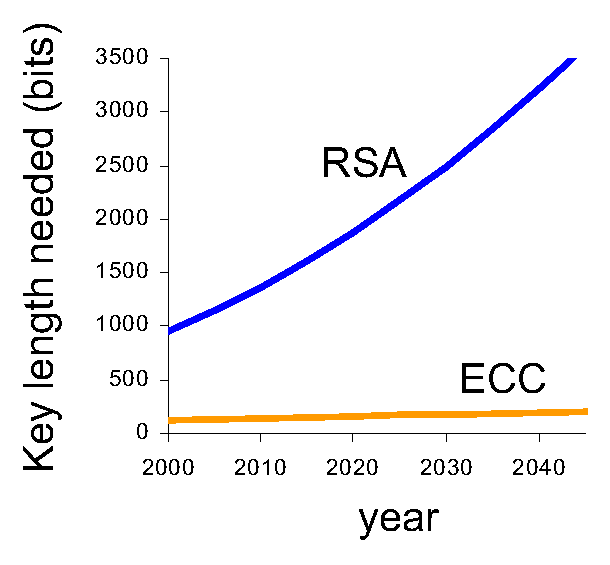
\includegraphics[scale=0.75]{figures/ThousandBitMultiplications}
\caption{Prognose of the key lengths to be regarded safe for RSA and
  Elliptic Curves\vspace{1ex}} 
\label{ThousandBitMultiplications}
\end{center}
\end{figure}

Nevertheless, thin clients like smart cards usually have to store the (long) secret key
and have to process a digital signature rather than to verify one. Therefore, there is
a clear advantage for ECC in terms of efficiency.
\par
\smallskip
Today, the major problem with ECC-implementations is the lack of standardization.
There is only one way to implement RSA, but there are many ways for ECC: One can work with
different sets of numbers, different (elliptic) curves described by up to 6 parameters,
and a variety of representations of the elements on the curve. Each choice has its
advantages and disadvantages, and one can certainly construct the most efficient for
each application. However, this causes problems in interoperability. But if all
ECC-tools should be able to communicate with each other, they will have to support
all different algorithms, which might put the advantage of efficient computation and
the need of less storage capacity to the contrary.

Therefore, international standardization organizations like IEEE (P1363),
ASC (ANSI X9.62, X9.63), ISO/IEC as well as major players like RSA labs or
Certicom have recently started standardization initiatives. While the IEEE
only describes the different implementations, the ASC has explicitly stated
10 elliptic curves and recommends their usage. The advantage of the ASC
approach is that one needs only a single byte to indicate which curve is
meant. However, it is not clear yet whether the ASC-curves will become a de
facto standard.

Although we see no need to replace RSA in any application today, one should
take the usage of ECC-based tools into consideration whenever a new system
is set up --- in particular, when the tool should be available beyond 2005.


\subsection{Elliptic curves --- history}

Mathematicians have been researching elliptic curves for over 100 years. In the
course of time, many lengthy and mathematically complex results have been found
and published in connection with elliptic curves. A mathematician would say that
elliptic curves (or the mathematics behind them) are widely understood. This
research was originally purely mathematical. That is to say, elliptic curves
were investigated, for example, in the mathematical areas of number theory and
algebraic geometry, which are generally highly abstract. Even in the recent
past, elliptic curves played an important role in pure mathematics. In 1993 and
1994, Andrew Wiles\index{Wiles} published mathematical works that triggered enthusiasm far
beyond the specialist audience. In these works, he proved a conjecture put
forward in the 1960's. To put it short, this conjecture was concerned with the
connection between elliptic curves and what are called module forms. That which
is interesting for most people is that the works of Wiles also proved the famous
second theorem of Fermat. Mathematicians had spent centuries (Fermat lived from
1601 to 1665) trying to find a strict proof of this theorem. Understandably,
therefore, Wiles' proof got a good response. Fermat formulated his theorem as
follows (written in the border of a book):

\begin{quote} {\em
Cubum autem in duos cubos, aut quadratoquadratum in duos quadratoquadratos, et
generaliter nullam in infinitum ultra quadratum potestatem in duos ejusdem
nominis fas est dividere: cujus rei demonstrationem mirabilem sane detexi. Hanc
marginis exiguitas non caperet.
} \end{quote}

Translated freely, using the denotation of modern mathematics, this means: \\
No positive whole numbers $x, y$ and $z$ greater than zero exist such that $x^n +
y^n = z^n$ for $n>2$. I have found an amazing proof of this fact, but there is
too little space in the border [of the book] to write it down.

This is truly amazing: A statement that is relatively simple to understand (we
are referring to Fermat's second theorem here) could only be proved after such a
long period of time, although Fermat himself claimed to have found a proof.
What's more, the proof found by Wiles is extremely extensive (all of Wiles
publications connected with the proof made up a book in themselves). This should
therefore make it obvious that elliptic curves are generally based on highly
complex mathematics.

Enough about the role of elliptic curves in pure mathematics. In 1985 Neal
Koblitz and Victor Miller independently suggested using elliptic curves in
cryptography. Elliptic curves have thus also found a concrete practical
application. Another interesting field of application for elliptic curves is for
factorising whole numbers. (For example the RSA cryptography system is based on
the \index{Complexity} difficulty/complexity of finding prime factors of an
extremely large number.) In this area, procedures based on elliptic curves have
been investigated and partially used since 1987 (a study by H.W. Lenstra). There
are also prime number tests based on elliptic curves.

Elliptic curves are used differently in the various areas. Encryption procedures
based on elliptic curves are based on the difficulty of a problem known as
elliptic curve discrete logarithm\index{Logarithm problem!discrete}. The factorisation of whole numbers uses the
fact that a large number of elliptic curves can be generated for a natural
composite number $n$ with several prime factors; however, these curves are not
then groups for composite $n$. \hyperlink{faktell}{More information about this
can be found under Factorisation using elliptic curves.}

\subsection{Elliptic curves --- mathematical basics}

This section provides information about \index{Group} {\em groups} and
\index{Field} {\em fields}.

\subsubsection{Groups}

Because the term {\em group} is used differently in everyday language than in
mathematics, we will, for reasons of completeness, begin by introducing the
essential statement of the formal definition of a group:
\begin{itemize}
   \item A group is a non-empty set $G$ and an operation $+.$ The set $G$ is
closed under the operation $+.$ Regardless of which two elements $a, b$ from $G$
are taken, performing the operation on them gives an element in $G$ (i.e.
$a+b=c$, and $c$ lies in $G$).
   \item For all elements $a, b$ and $c$ in $G$: $(a+b)+c = a+(b+c)$.
   \item There exists an element $e$ in $G$ that behaves neutrally with respect
to the operation $+$. That means that for all a in the set $G: ~a+e = e+a = a.$
   \item For each element $a$ in $G$ there exists a so-called inverse element $-a$
($-a$ also lies in $G$) such that: $a+(-a) = (-a)+a = e$.
\end{itemize}
If also $a+b = b+a$ for all $a, b$ in $G$ then we call the group an {\em
Abelian} group. An operation denoted as $+$ indicates an {\em additive} group;
if the operation is denoted as $\cdot$, we speak of a {\em multiplicative}
group.

The simplest example of an (Abelian) group is the group of whole numbers under
the standard operation of addition. The set of whole numbers is denoted as
${\mathbb Z}$. ${\mathbb Z}$ has an infinite number of elements, because
${\mathbb Z} = \{ \cdots, -4, -3, -2, -1, 0, 1, 2, 3, 4, \cdots\}$. For example, the
operation of $1+2$ lies in ${\mathbb Z}$, for $1+2 = 3$ and $3$ lies in
${\mathbb Z}$. The neutral element in the group ${\mathbb Z}$ is $0$. The
inverse element of $3$ is $-3$, for $3+(-3) = 0$.

There are also {\em finite} groups. This means that these exists a set
$\mathcal{M}$ with a fixed number of elements and an operation $+$ such that the
above conditions are fulfilled. One example of this is any set ${\mathbb Z}_n$
where ${\mathbb Z}_n = \{0, 1, 2, 3, \cdots, n-1\}, n$ is a positive whole number
and the operation is addition mod $n$, i.e. $a$ and $b$ in ${\mathbb Z}_n$ are
subject to the operation $a+b \;{\rm mod~} n$.

\paragraph{Cyclic groups}
Cyclic groups\index{Group!cyclic} are those groups $G'$ that possess an element $g$
from which the group operation can be used to generate all other
elements in the group. This means that for each element $a$ in
$G'$ there exists a positive whole number $i$ such that if $g$ is
subject to the operation $i$ times (i.e. ``$g \cdot i$''),
$g+g+\cdots+g = a$ (additive group) or $g^i = g\cdot g \cdots g = a$
(multiplicative group). The element $g$ is the {\em generator} of
the cyclic group --- each element in $G�$ can be generated using
$g$ and the operation.

Now to the order of an element of the group: Let $a$ be in $G$. The smallest
positive whole number $r$ for which $a$ subject to the operation with itself $r$
times is the neutral element of the group $G�$ (i.e.: $r \cdot a = a+a+\cdots+a =
e$ bzw.\ $a^r = e$), is called the {\em order} of $a$.

The order of the group is the number of elements in the set $G$.

\subsubsection{Fields}

In mathematics, a field is understood to be a set $K$ with two operations
(denoted as $+$ and $\cdot$) which fulfils the following conditions:
\begin{itemize}
   \item The set $K$ forms an Abelian group together with the operation $+$
(addition), where $0$ is the neutral element of the operation $s$.
   \item The set $K$ (without the element 0) also forms an Abelian group
together with the operation $\cdot$ (multiplication).
   \item For all elements $a, b$ and $n$ in $K$, $n\cdot (a+b) = n \cdot a + n
\cdot b$ and $(a+b) \cdot n = a \cdot n + b \cdot n$.
\end{itemize}

There are {\em infinite} fields, i.e. the set on which the field is based
contains an infinite number of elements (e.g.: the field of real numbers). And
there are also finite fields, such as ${\mathbb Z}_p = \{0, 1, 2, 3, \cdots, p-1\}$
, where $p$ is a prime. ${\mathbb Z}_p$ with addition mod $p$ and multiplication
mod $p$ is a finite field.
\index{Field!Characteristic}
\paragraph{Characteristic of a field}
Let $K$ be a field and $1$ be the neutral element of $K$ with
respect to the multiplicative operation ``$\cdot$''. For positive
natural numbers $n$, let us understand $n_1$ to be $n_1 = 1 + 1 +
\cdots + 1$ ($n$ summands and $n_1$ is an element in $K$). If $n_1$
is then unequal to $0$ for all $n>0$, then we call $K$ a field
with characteristic zero. Otherwise, the characteristic of $K$ is
defined to be the smallest positive natural number $p$ for which
$p_1 = 0$ (note: $p$ is then a prime). Comment: The field of real
numbers has the characteristic $0$; the field ${\mathbb Z}_p$ has
the characteristic $p$.

\subsection{Elliptic curves in cryptography}

An elliptic curve is described by an equation. In order to keep it simple, we
restrict our explanation to elliptic curves over $${\mathbb Z}_p = \{0, 1, 2, 3,
\cdots, p-1\}$$ where $p$ is a prime greater than $3$. ${\mathbb Z}_p$ with
addition mod $p$ and multiplication mod $p$ is a finite field. However, we must
mention that elliptic curves can be defined over any (finite) field. In
particular, elliptic curves over fields with characteristic $2$ are extremely
interesting from a practical point of view because computers can be used to
represent the elements from these fields as bit strings. This leads to an
efficient implementation of the arithmetic in such fields, which means that a
computer can perform the operations of the field particularly quickly.

Because these points actually refer to the same thing, it is seldom necessary to distinguish between exact meanings.

An elliptic curve over ${\mathbb Z}_p$ is defined by an equation of the following form:
$$ y^2 \; ({\rm mod} \; p) = x^3 + ax + b ({\rm mod} \; p) $$
(thus: equality in the field ${\mathbb Z}_p$), where $a, b$ are in ${\mathbb Z}_p$ and $4a^3 + 27b^2$ mod $p$ is
not equal to zero. For fixed chosen numbers $a$ and $b$ in ${\mathbb Z}_p$, this equation has the pair of solutions
$$ {\bf E} = \left\{(x,y) \left| \begin{array}{c} x {\rm ~and~} y {\rm ~are~in~} {\mathbb Z}_p {\rm ~and~} \\
y^2  \equiv x^3 + ax + b \;({\rm mod~} p) {\rm ~and~} \\ 4a^3 + 27b^2 \not\equiv 0 \;
({\rm mod~} p)\end{array} \right. \right\}, $$ i.e. the set ${\bf E}$ consists of all pairs $x$ and $y$ that are a solution
(in ${\mathbb Z}_p$) of the above equation. It must be noted that the numbers $a, b$ and $p$ determine which pairs $(x,y)$
lie in the set ${\bf E}$. This means that $a, b$ and $p$ specify this set. The elements $(x,y)$ in ${\bf E}$ are called
points on the elliptic curve. In addition, ${\bf E}$ has one more element $O$ (the so-called point in infinity).
The set ${\bf E}$ is usually called an elliptic curve. 

We can now define an operation\footnote{A animated addition of elliptic curve points can be
found at the web page of Certicom\index{Certicom}:
\href{http://www.certicom.com/resources/ecc_tutorial/ecc_tutorial.html}{\tt http://www.certicom.com/resources/ecc\_tutorial/ecc\_tutorial.html}.}
(also denoted as $+$, although it is
not the standard/usual addition of real numbers) on two elements in ${\bf E}$ such that the operation delivers an element
that also lies in ${\bf E}$. The set ${\bf E}$ is therefore closed under the operation $+$. We can show
that ${\bf E}$ is a group. The neutral element of the group ${\bf E}$ is the point in infinity $O$. Thus, for every two
points $(x_1,y_1)$ and $(x_2,y_2)$ on the elliptic curve ${\bf E}$, there exists a point $(x_3,y_3)$ on ${\bf E}$ such that
the operation $+$ complies with the following: $(x_1,y_1) + (x_2,y_2) = (x_3,y_3)$. Under certain circumstances, these points
may also be equal to the point in infinity. Thus, when we speak of a point $P$ on an elliptic curve ${\bf E}$,
we mean that $P = (x,y)$ and $(x,y)$ lies in the set ${\bf E}$. Any two points on an elliptic curve specified by $a, b$ and $p$
can therefore be added and the result is a point that also lies on the same elliptic curve.

% \newpage
\begin{figure}[htbp]
\subsubsection*{Adding of two points on an elliptic curve}
The following two figures show an elliptic curve in the affine plane and
shows how points on an elliptic curve are added. Note that the point in infinity $O$ cannot be represented in
the affine plane.
\begin{center}
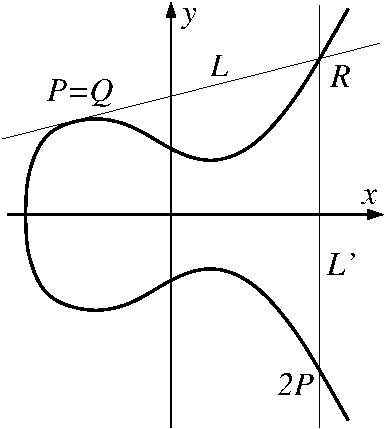
\includegraphics[scale=1.08]{figures/ec-mult2}
\caption{Doubling the point P} \vspace{\floatsep} \vskip +20 pt
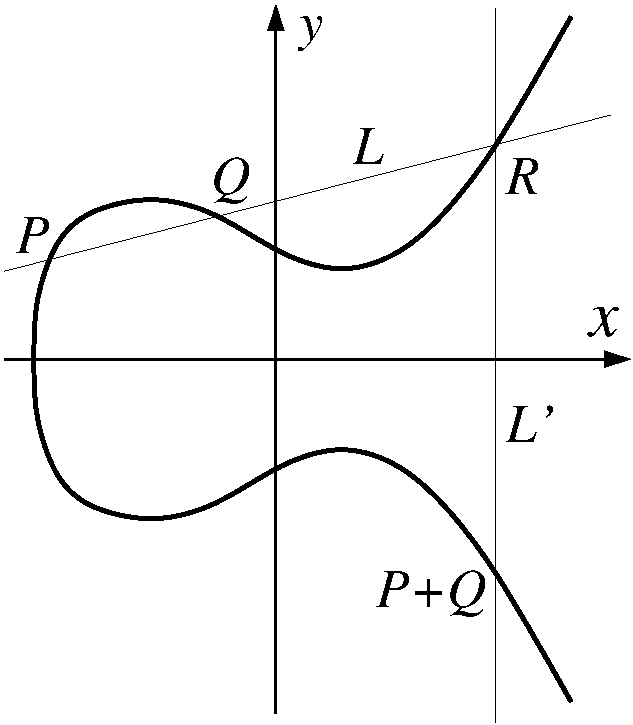
\includegraphics[scale=0.65]{figures/ec-add}
\caption{ Adding distinct points P and Q} % \footnotemark}
\end{center}
\end{figure}
% \addtocounter{footnote}{0}\footnotetext{The point $O$ cannot be represented in the affine plane.}
\enlargethispage{+20pt}

\newpage
We must note that ${\bf E}$ can have the following meanings:
\begin{itemize}
   \item the set ${\bf E}$ of solutions pairs $(x,y)$ for an equation including the point $O$
   \item the group ${\bf E}$ (with the operation ``addition of $(x_1,y_1)$ and $(x_2,y_2)$'')
   \item the elliptic curve ${\bf E}$ (which is actually the same as the group ${\bf E}$)
\end{itemize}
For cryptography, the important fact is that, for very large numbers, it appears to be extremely difficult to use a
given point $Q$ on an elliptic curve to determine which two points have to be added to obtain $Q$.

For large numbers $a, b$ and $p$ ($p$, for example, has a length of more than $160$ bits), the computer can easily add
the point $P$  $m$ times after another, i.e. to determine the point $P + P + \cdots + P = Q$ in an incredibly short space
of time (in a few fractions of a second) ($m$ summands $P$). Rather than $P + P + \cdots + P = Q$ ($m$ summands $P$)
we also write $mP = Q$. If we have a point $P$ and a point $Q$, which both lie on the same elliptic curve, no procedure
is known that enables us --- within an acceptable space of time --- to determine the number $m$ (assuming it actually exists)
for which $mP = Q$. This is referred to as the ``elliptic curve discrete logarithm problem'' (abbreviated to ECDLP)\index{ECDLP}.

We must note that not all elliptic curves are equally secure. This
means that we must choose the parameters $a$ and $b$ carefully
when defining a curve. For certain classes of elliptic curves, it
is possible to solve the ECDLP easier than in the general case.
Cryptographically unsuitable elliptic curves are called {\em abnormal}
curves (these are curves over ${\mathbb Z}_p$ for which the set
${\bf E}$ has precisely $p$ elements) and the {\em supersingular} curves
(the curves for which we can reduce the calculation of the ECDLP
to calculating the ``standard'' discrete logarithm in other finite
fields, i.e. simplify the calculation). There are therefore
cryptographically good and bad curves. However, for given
parameters $a$ and $b$ we can, with some difficulty, establish
whether or not the resulting elliptic curve is useful for
cryptographic purposes. The curves used in cryptography are
usually provided by experts. They ensure that the elliptic curves
they classify as secure satisfy the current security requirements.

For secure curves, the parameter $p$ determines how long it takes
to solve the ECDLP on this curve. The larger the parameter $p$,
the longer it takes to solve the problem. Experts recommend a bit
length of over $200$ bits for the parameter $p$. This makes it
clear why elliptic curves are so interesting for cryptography.
Because the parameter $p$ also determines the time required to
perform the signature/encryption procedure when using elliptic
curves in cryptography. The time taken to generate a pair of keys
also depends on $p$. Thus, small values (few bits) are desirable
here (in order to minimise the run times for the procedures);
however, the required security must still be maintained. For
example, with a length of $200$ bits for $p$, a {\em good}
elliptic curve is just as secure as an \index{RSA!module} RSA
module of over $1024$ bits in length (at least according to the
current state of research). The reason for this is that the
quickest algorithms for solving the {\em elliptic curve discrete
logarithm} problem have an exponential run time --- unlike the
subexponential run times that the best factorisation algorithms
currently have (number sieve, quadratic sieve or factorisation
with elliptic curves). Therefore, the parameters for cryptographic
procedures based on the problem of {\em factorising whole numbers}
must be greater than the parameters for cryptographic procedures
based on the ECDLP problem.

\subsubsection{Digital signatures using elliptic curves}

The {\em elliptic curve discrete logarithm problem} (ECDLP) \index{ECDLP} forms the basis for
elliptic-curve cryptography. Various signature procedures are based on this.
What they have in common is how they use the public parameters and how these
parameters are used to generate secret and public keys:
\begin{itemize}
    \item The parameters of the elliptic curve E, i.e. a prime number $p$ that
determines over which field ${\mathbb Z}_p$ the elliptic curve ${\bf E}$ is
defined, as well as the two numbers $a$ and $b$ in ${\mathbb Z}_p$.
    \item A point $G=(x,y)$ that lies on the elliptic curve ${\bf E}$.
    \item A prime number $r < p$ for which $rG=O$ (i.e. $G$ added $r$ times
gives the neutral element of the group ${\bf E}$) and $r$ is a factor of $\#{\bf
E}$ (where $\# {\bf E}$ is the number of elements in the set ${\bf E}$). The
point $G$ therefore has the order $r$ and is the generator of a cyclic subgroup
of ${\bf E}$ with the order $r$.
    \item The number $k = \#{\bf E}/r$ ($k$ is called the {\em cofactor}).
\end{itemize}
The parameters $a, b, p, G, r$ and $k$ listed above are called
{\em domain parameters}.\index{Domain parameters} They determine on which elliptic curve ${\bf
E}$ and in which cyclic subgroup of ${\bf E}$ a signature
procedure has been ``used''.

The secret key $s$ of the signature generator is a (random) whole number $s$ in
the interval $[1, r-1]$. The public key of the signature generator is a point
$W=(x,y)$ on the elliptic curve ${\bf E}$. The public key $W$ and secret key $s$
are interrelated as follows: $W = sG$. This means that the domain parameters
(particularly $G$) and the secret key $s$ are used to calculate the public key
$W$ (by adding $G$ $s$ times on ${\bf E}$). The ECDLP is obviously used here: If
$W$ and $G$ (as well as the other domain parameters used) are known, then it is
difficult to use these to calculate $s$. (If the parameters are chosen
correctly, this currently appears to be practically impossible).

In order to verify a signature, the recipient of the signature must know the
following:
\begin{enumerate}
   \item The signature procedure used,
   \item The hash function used,
   \item The domain parameters used to generate the signature
   \item The public key $W$ of the signature generator.
\end{enumerate}


\subsubsection{Factorisation using elliptic curves}

\hypertarget{faktell}{}

There are factorisation algorithms based on elliptic curves\footnote{In 1987 H.W. Lenstra published
a factorisation algorithm, based on elliptic curves (see \cite{Lenstra1987}).
The biggest compound number curently factorised with elliptic curves is the number $ 628^{59}-1, $ which has 55 decimal digits. It was
found Oct. 6th, 2001 by M. Izumi (See \hyperlink{Lenstra2}{ECMNET}\index{ECMNET}).
}. More precisely,
these procedures exploit the fact that elliptic curves can be defined over
${\mathbb Z}_n$ ($n$ composite number). Elliptic curves over ${\mathbb Z}_n$ do
not form a group, because not every point on such an elliptic curve has an
inverse point. This is connected with the fact that - if $n$ is a composite
number - there exist elements in ${\mathbb Z}_n$ that do not have an inverse
with respect to multiplication mod $n$. In order to add two points on an
elliptic curve over ${\mathbb Z}_n$, we can calculate in the same way as on
elliptic curves over ${\mathbb Z}_p$. Addition of two points (on an elliptic
curve over ${\mathbb Z}_n$), however, fails if and only if a factor of $n$ has
been found. The reason for this is that the procedure for adding points on
elliptic curves gives elements in ${\mathbb Z}_n$ and calculates the inverse
elements for these (with respect to multiplication mod $n$) in ${\mathbb Z}_n$.
The extended \index{Euclidean algorithm} Euclidean algorithm is used here. If
the addition of two points (that lie of an elliptic curve over ${\mathbb Z}_n$)
gives an element in ${\mathbb Z}_n$ that does not have an inverse element in
${\mathbb Z}_n$, then the extended Euclidean algorithm delivers a genuine factor
of $n$.

Factorisation using elliptic curves thus principally works as follows: You
select random curves over ${\mathbb Z}_n$, as well as random points (that lie on
this curve) and add them; you thus obtain points that also lie on the curve or
find a factor of $n$. Factorisation algorithms based on elliptic curves
therefore work probabilistically. The opportunity of defining large number of
elliptic curves over ${\mathbb Z}_n$ allows you to increase the probability of
finding two points which you can add to obtain a factor of $n$. These procedures
are therefore highly suitable for parallelisation.

\subsection{Implementing elliptic curves}

CrypTool uses elliptic curves for the digital signature function.

It implements the basic algorithms for group operations, for generating elliptic
curves, for importing and exporting parameters for elliptic curves over finite
fields with $p$ ($p$ prime) elements. The algorithms have been implemented in
ANSI C and comply with draft no. 8 of the IEEE P1363 work group {\em Standard
Specifications for Public Key Cryptography}

{\href{http://grouper.ieee.org/groups/1363}{\tt
http://grouper.ieee.org/groups/1363}}.

The procedure implements the cryptographic primitives for generating and
verifying signatures for the variations of Nyberg-Rueppel signatures and
\index{DSA} DAS signatures based on elliptic curves (in accordance with draft
no. 8 of the IEEE P1363 work group). This was done in collaboration with the
SECUDE GmbH --- using the above library and the SECUDE SDK.
\index{SECUDE GmbH}

\newpage
%\addcontentsline{toc}{subsection}{Literaturverzeichnis}
\begin{thebibliography}{99999}
\addcontentsline{toc}{subsection}{Bibliography}
        \bibitem[Lenstra1987]{Lenstra1987} H.W. Lenstra\\ \index{Lenstra 1987}
                Factoring integers with elliptic curves, Annals of Mathematics 126, pp. 649-673, 1987.
\end{thebibliography}
%\newpage

\section*{Web links}\addcontentsline{toc}{subsection}{Web links}

\begin{enumerate}
   \item Certicom � Online Tutorial, \index{Certicom}\\
                \href{http://www.certicom.com/resources/ecc_tutorial/ecc_tutorial.html}{\texttt{http://www.certicom.com/resources/ecc\_tutorial/ecc\_tutorial.html}}
        \item IEEE P1363

                \href{http://grouper.ieee.org/groups/1363}{\texttt{http://grouper.ieee.org/groups/1363}}
        \item  \hypertarget{Lenstra2}{}
An informative web page to the factorisation with elliptic curves.

\href{http://www.loria.fr/~zimmerma/records/ecmnet.html}{\texttt{http://www.loria.fr/\~{}zimmerma/records/ecmnet.html}}

There, one finds literature to the topic factorisation with elliptic curves as well as link to other web page. 

\end{enumerate}

